\begin{minipage}[t]{180mm}
\fcolorbox{black}{white}{
\begin{minipage}[b]{30mm}

\includegraphics[width=0.5\linewidth]{unflogo.pdf}
\end{minipage}
\begin{minipage}[b]{100mm}
\Huge \textbf{UNF NEWZ} \\
\Large -- Søvn og retsstavning er overvurderet! 
\end{minipage}
\begin{minipage}[b]{50mm}
\Large Onsdag 17.07.2015 \\
\normalsize Redigeret i \LaTeX\ af \\ SOM, MGS, MMN, SABH
\end{minipage}
}
\end{minipage}



\begin{minipage}[b]{0.95\linewidth}
\begin{minipage}[t]{0.47\textwidth}
\vspace{3mm}
\section*{RUC -- \\ Revolutionen Udsættes i Cirkus}
Et bud har overbragt os gode nyheder fra kongernes gravby. Ungdommen er ikke så rådden som de sidste år, og der er derfor færre der har besluttet at opfre deres intellekt på hippiernes malformede altar. Denne nyhed varmer selvfølgelig vores hjerter, og føder en spinkel tanke, om at verden måske alligevel ikke er gået helt til lave. Desværre virker det som om hippierne har fundet på nye tiltag, for at tiltrække flere ofre det deres fordumningsmaskine:
\begin{itemize}
\item Campus flyttes fra Roskilde til Thylejren.
\item Der udleveres gratis hash hver mandag morgen på alle landets ungdomsuddannelser.
\item
\item
\item
\item
\end{itemize}

\end{minipage}
\hfill\begin{minipage}[t]{0.47\textwidth}

\vspace{1mm}
\tikzstyle{mybox} = [draw=white, fill=blue!20, very thick,
    rectangle, rounded corners, inner sep=10pt, inner ysep=20pt]
\tikzstyle{fancytitle} =[fill=red, text=white]

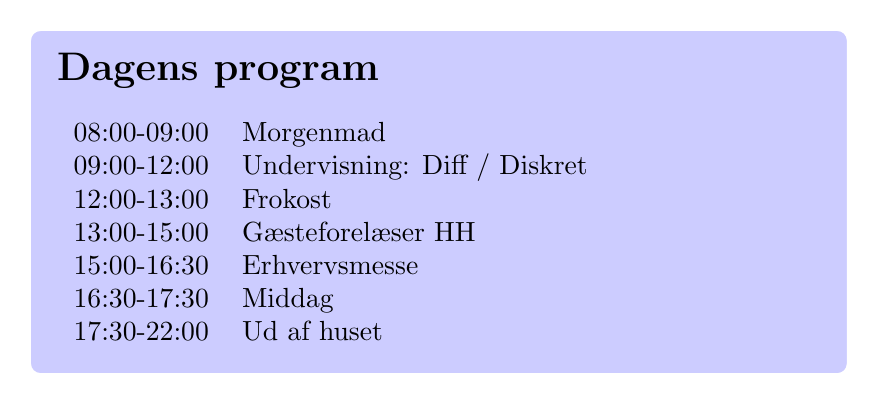
\begin{tikzpicture}
\node [mybox] (box){%
\begin{minipage}{0.80\textwidth}
\vspace{-4mm}\section*{Dagens program}
\begin{tabular}{ll}
08:00-09:00 & Morgenmad \\
09:00-12:00 & Undervisning: Diff / Diskret \\
12:00-13:00 & Frokost \\
13:00-15:00 & Gæsteforelæser HH \\
15:00-16:30 & Erhvervsmesse \\
16:30-17:30 & Middag \\
17:30-22:00 & Ud af huset
\end{tabular}
\vspace{-4mm}
\end{minipage}
};
\end{tikzpicture}%

\section*{Ninjas dagbog}
Dagen idag kommer til ikke at have været lige så tilfredsstillende som den i går, da jeg ikke vil have dræbt lige så mange koordinatorer. Som erstatning vil jeg dog hen imod aften have fået muligheden for at skære i dusinvis af små børn, og gøde blomster med deres blod, men forventningens glæde forsvinder fra deres øjne.

Dette vil dog ikke have været lige så hyggeligt som gårdsdagens drab, da hverken de hyperaktive småbørn eller deres hipsterforældre var i stand til at gøre synderlig modstand, og på trods af deres påståede individualtitet kom de alle med det samme klynkeri om ønsket fortsat ovelevelse, og kun de færreste vil have tilbudt at ofre dem selv for at forlænge deres børns liv. 

Disse ønsker vil jeg selvfølgeligt have opfyldt, ved at dræbe forældrene mens deres børn så på, modsat min almidelige strategi i hvilken jeg vil have dræbt børnene foran deres forældre, da dette vil have virket mere passende, eftersom børneblod er bedre til at dyrke røde roser.

{\flushright\emph{Ninja,lidt høj på blod}}

\vspace{2mm}

\includegraphics[width=\linewidth]{wewantyou.jpg}

\end{minipage}
\end{minipage}
